\label{sec:failure-modes}

Across this audit and its immediate predecessor experiments, we observed several bounded,
marker-specific interactions in frozen correlated settings. Their directions were mixed, and
the comparisons do not establish independent, causal, or universal properties of frozen
pathology foundation-model embeddings. Each observation is tied to its specific empirical
configuration rather than presented as an abstract general law.
Accordingly, Gate A did not overturn the prior directional observations; it bounds
generalizability across configuration, endpoint, encoder, and site, and insufficient evidence
is treated as unresolved rather than contrary evidence.

\subsection{Scale, tile sampling, and encoder interact within a correlated grid}

The obsolete 90-slide, three-marker, single-seed diagnostic has been replaced by the completed
frozen Gate A grid. It contains 360 correlated seed-level cells across six markers, two
encoders, 16/32/64 tiles, five sampling seeds, and encoder-specific native versus shared
$1.76\,\mu$m/px scales. These are summarized into 72 five-seed configurations and 390 paired
contrasts. All settings reuse frozen cohorts and folds: they are neither independent
replications nor 360 confirmatory tests, and the sampling-seed Student-$t$ intervals in
Figure~\ref{fig:scale-heatmap} are not patient-level confidence intervals.

SPOP shows the largest instability: AUROC spans 0.348--0.679, 25/60 seed-level cells are
chance-or-worse, 8/12 configuration seed ranges straddle chance, 19/30 native-scale pairs
cross the null, and 4/15 shared-scale encoder pairs cross it. It is unsupported in the frozen
primary configuration and configuration-sensitive in Gate A: neither a robust positive nor a
robust null is established, and a modest effect and tumor dilution remain unresolved. AR is
positive in all 60 cells ($\rho=0.136$--$0.297$), so its positive pooled direction is consistent
across the correlated Gate A settings, while site heterogeneity and transportability are neither
supported nor refuted. Its grade-independent increment remains unresolved, and no scanner,
stain, or site causality is inferred. Marker 7 has CONCH configuration means of 0.681--0.739
and Virchow means of 0.545--0.658; Virchow's
shared-$1.76\,\mu$m/px means are 0.634--0.658 versus 0.545--0.557 at native
$0.44\,\mu$m/px, and one of 60 cells is chance-or-worse. Because source retention varies
from 498 to 502 patients, R2 repeated all 60 cells on the common 498-patient source. It found
zero raw-to-common null crossings and preserved all 65 paired contrast directions; individual
C-indices shifted by $-0.0023$ to $+0.0229$. This does not explain or reverse the observed
directions, establish a causal scale effect, or demonstrate universal encoder superiority.
Official PFI is complete: C-index 0.586 (95\% CI 0.482--0.689), with the interval including
0.5. Gleason, phenotype, and PTEN each have zero chance-or-worse cells, but
that fact alone does not elevate their tiers or constitute external validation. C04/C05
R5 evidence closure is complete while their scientific interpretations remain unresolved.

\begin{figure}[htbp]
\centering
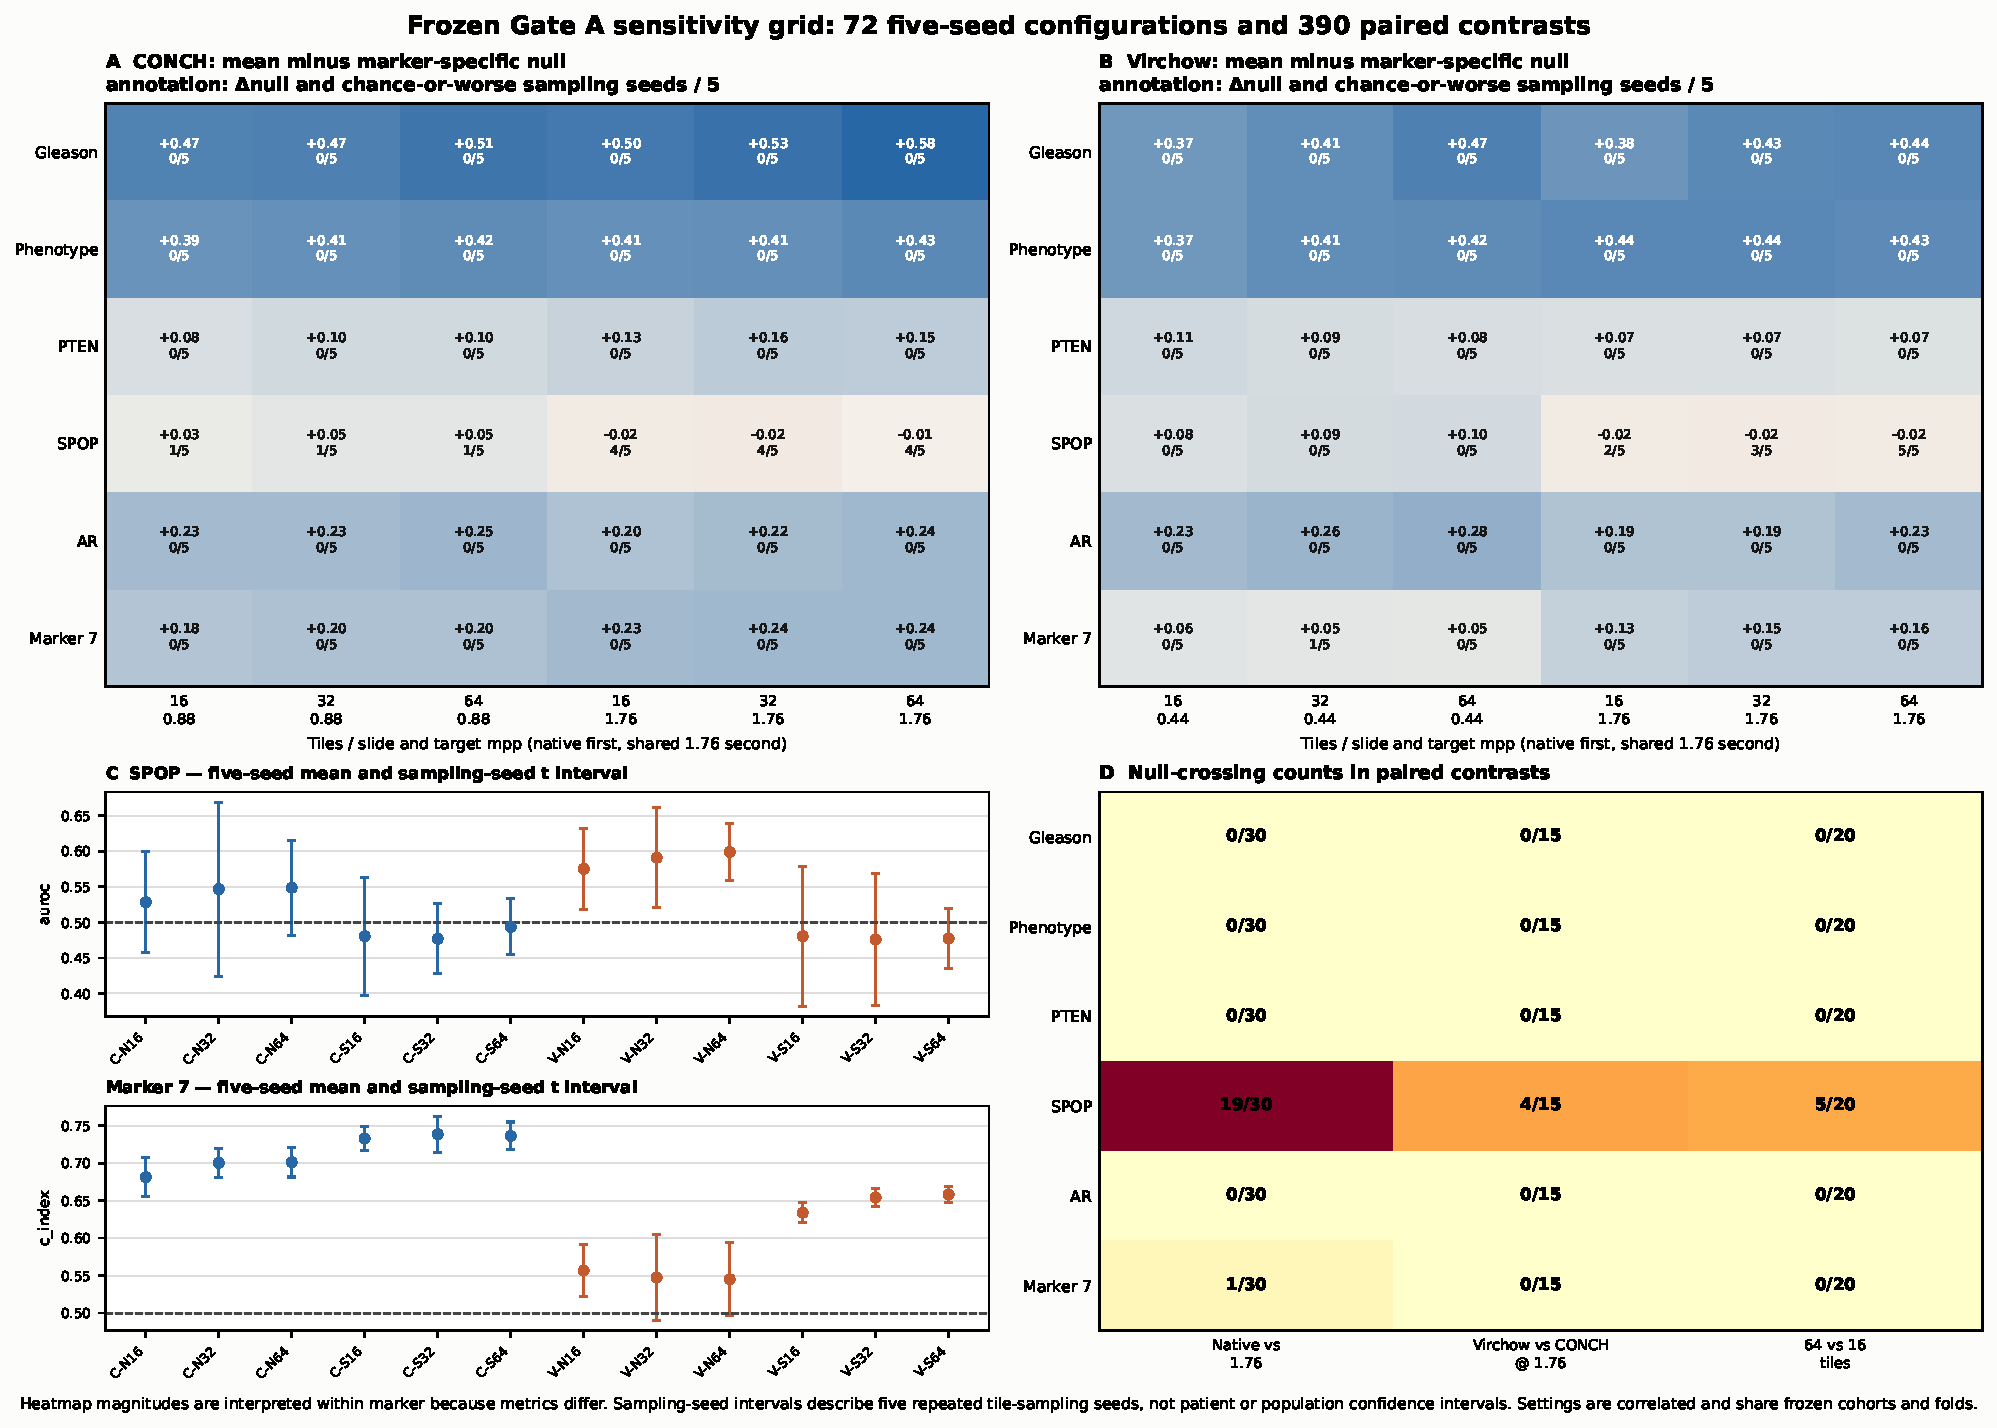
\includegraphics[width=0.95\textwidth]{figures/fig9_scale_tile_heatmap.pdf}
\caption{Frozen Gate A correlated sensitivity grid. (A--B) CONCH and Virchow five-seed means
minus each marker-specific null, with the chance-or-worse seed count in each cell; magnitudes
are interpreted within marker because metrics differ. (C) SPOP and marker-7 means with
sampling-seed Student-$t$ intervals, which are not patient confidence intervals. (D) Null-
crossing count/denominator for three paired contrast types. All settings share frozen cohorts
and folds.}
\label{fig:scale-heatmap}
\end{figure}

\subsection{Different encoders can show different descriptive transfer patterns}

Marker 7 provides the clearest post-hoc descriptive observations: CONCH is higher in
the current grid, while Virchow improves at the shared $1.76\,\mu$m/px scale. Its effect size
and transfer generalizability are limited by endpoint, encoder, and scale. Common-498 R2 and
official-PFI R3 are complete. A single-encoder cross-cohort
result cannot establish a generally transferable prognostic marker or distinguish it from a
setting-specific fitted direction. These observations are not proof of prognostic validity, a
causal mechanism, or a probability of chance discovery. The counter-case is also informative:
the PTEN/AR nested
confounder-audit increments (Section~\ref{sec:confounder-audits}) \emph{converge} across CONCH
and Virchow rather than diverging, providing descriptive cross-encoder convergence for their
weak, uncertain increments rather than proof of a universal property. Cross-encoder replication
can therefore inform both a claimed positive result and an unsupported or uncertain result
without changing the evidentiary status by itself.

\subsection{Qualification against one target does not certify transfer to a different downstream outcome}

Exploratory in-cohort discrimination was observed after refitting in the same embedding space
(Section~\ref{sec:leopard-results}), while qualified grade, phenotype, PTEN, and AR markers did
not predict LEOPARD's recurrence outcome better than chance. This post-hoc descriptive contrast
does not establish prognostic validity or quantify chance discovery; it shows only that
qualification for one target did not certify transfer to the tested downstream outcome.

\subsection{Hyperparameter choices can flip borderline results}

Standardizing a single protocol across all 13 originally tested hypotheses (Section~\ref{sec:gates})
changed one candidate (TCGA-PRAD H\&E$\to$ERG fusion status) from nominally significant to
null; we adopt the standardized number as authoritative throughout and flag this as a reason to
distrust single-protocol borderline claims in general.

\subsection{Label and outcome definitions are not interchangeable across cohorts even under the same name}

TCGA-PRAD's GDC-harmonized clinical data has no populated \texttt{days\_to\_recurrence} field
for this cohort; a recurrence-style label reconstructed from
\texttt{follow\_ups.disease\_response} is a coarser, clinical-assessment-based construct than
LEOPARD's explicit PSA-based biochemical-recurrence definition or TCGA's own standardized
PFS/DFS endpoints, and marker 7's attenuated transfer to those standard endpoints
(Section~\ref{sec:res-label-benchmark}) should be read as evidence of this pitfall in action,
not as a separate failure.
